\PassOptionsToPackage{unicode}{hyperref}
\PassOptionsToPackage{naturalnames}{hyperref}

\documentclass[10pt]{beamer}

\usetheme[sectionpage=none,block=fill]{metropolis}

\usepackage{acronym} % \ac[p], \acl[ptl], \acs[p], \acf[p]
\usepackage{algorithm, algpseudocode}
\usepackage{appendixnumberbeamer}
\usepackage[backend=biber,style=alphabetic,sorting=none,maxbibnames=1]{biblatex}
\usepackage{amsmath, amssymb, amsthm}
\usepackage[french]{babel}
\usepackage{bookmark}
\usepackage{booktabs} % \toprule, \midrule, \cmidrule, \bottomrule
\usepackage{cancel} % \cancel
\usepackage{caption}
\usepackage[scale=2]{ccicons}
\usepackage{csquotes} % Dépendance de babel
\usepackage{graphicx}
\hypersetup{hidelinks}
% \usepackage[inline]{enumitem}
% \setlist[enumerate]{label=(\roman*)} %% <- set the base level label separately
\usepackage{marvosym} % \Flatsteel
\usepackage{MnSymbol} % \dashrightarrow
\usepackage{pifont} % \ding
\usepackage{silence} % \WarningFilter
\WarningFilter{biblatex}{Patching footnotes failed}
\usepackage{subcaption} % subfigure
\usepackage{tikz} % \begin{tikzpicture} \end{tikzpicture}
\usetikzlibrary{calc}
\usetikzlibrary{graphs}
\usetikzlibrary{positioning}
\usetikzlibrary{quotes}
\usetikzlibrary{shapes.misc}
\usetikzlibrary{tikzmark}
\usepackage{wasysym} % \checked
\usepackage{xcolor}
\usepackage{xspace} % \xspace

%-------------------------------------------------------------------
%                           Assets
%-------------------------------------------------------------------
\acrodef{ADT}[ADT]{Abstract Data Type}
\acrodefplural{ADT}[ADTs]{Abstract Data Types}
\acrodef{API}[API]{Application Programming Interface}
\acrodef{AW}[AW]{Add-Wins}
\acrodef{CCI}[CCI]{Convergence, Causality preservation, Intention preservation}
\acrodef{CL}[CL]{Causal-Length}
\acrodef{CRDT}[CRDT]{Conflict-free Replicated Data Type}
\acrodefplural{CRDT}[CRDTs]{Conflict-free Replicated Data Types}
\acrodef{DAG}[DAG]{Directed Acyclic Graph}
\acrodef{FIFO}[FIFO]{First In, First Out}
\acrodef{GC}[GC]{Garbage Collection}
\acrodef{IPFS}[IPFS]{InterPlanetary File System}
\acrodef{JIT}[JIT]{Just-In-Time}
\acrodef{LCA}[PPAC]{Plus Petit Ancêtre Commun}
\acrodef{LFS}[LFS]{Local-First Software}
\acrodef{LUB}[LUB]{Least Upper Bound}
\acrodef{LWW}[LWW]{Last-Writer-Wins}
\acrodef{MUTE}[MUTE]{Multi User Text Editor}
\acrodef{MV}[MV]{Multi-Value}
\acrodef{OC}[OC]{Commutativité des Opérations}
\acrodef{OT}[OT]{Operational Transformation}
\acrodefplural{OT}[OT]{Operational Transformations}
\acrodef{P2P}[P2P]{pair-à-pair}
\acrodef{PKI}[PKI]{Public Key Infrastructure}
\acrodef{PoC}[PoC]{Proof of Concept}
\acrodef{PT}[PT]{Transitivité de la Précédence}
\acrodef{RADT}[RADT]{Replicated Abstract Data Type}
\acrodefplural{RADT}[RADTs]{Replicated Abstract Data Types}
\acrodef{RCB}[RCB]{Reliable Causal Broadcast}
\acrodef{RGA}[RGA]{Replicated Growable Array}
\acrodef{RW}[RW]{Remove-Wins}
\acrodef{SEC}[SEC]{Cohérence forte à terme}
\acrodef{SPOF}[SPOF]{Single Point Of Failure}
\acrodef{TTF}[TTF]{Tombstone Transformation Function}
\acrodefplural{TTF}[TTF]{Tombstone Transformation Functions}
\acrodef{WebRTC}[WebRTC]{Web Real-Time Communication}

\floatname{algorithm}{Algorithme} % Renomme caption de "Algorithm" -> "Algorithme"

\newcommand\CONDITION[2]%
  {\begin{tabular}[t]{@{}l@{}l@{}}
     #1&#2
   \end{tabular}%
  }
  \algdef{SE}[WHILE]{While}{EndWhile}[1]%
  {\algorithmicwhile\ \CONDITION{#1}{\ \algorithmicdo}}%
  {\algorithmicend\ \algorithmicwhile}
\algdef{SE}[FOR]{For}{EndFor}[1]%
  {\algorithmicfor\ \CONDITION{#1}{\ \algorithmicdo}}%
  {\algorithmicend\ \algorithmicfor}
\algdef{S}[FOR]{ForAll}[1]%
  {\algorithmicforall\ \CONDITION{#1}{\ \algorithmicdo}}
\algdef{SE}[REPEAT]{Repeat}{Until}{\algorithmicrepeat}[1]%
  {\algorithmicuntil\ \CONDITION{#1}{}}
\algdef{SE}[IF]{If}{EndIf}[1]%
  {\algorithmicif\ \CONDITION{#1}{\ \algorithmicthen}}%
  {\algorithmicend\ \algorithmicif}%
\algdef{C}[IF]{IF}{ElsIf}[1]%
  {\algorithmicelse\ \algorithmicif\ \CONDITION{#1}{\ \algorithmicthen}}

\newcommand{\commentbott}{with $\bott$ the minimal tuple}
\newcommand{\commenttopt}{with $\topt$ the maximal tuple}

\newcommand{\algorithmautorefname}{Algorithme}
\newcommand{\annexautorefname}{Annexe}
\newcommand{\definitionautorefname}{Définition}
\newcommand{\propertyautorefname}{Propriété}
% \newcommand{\subfigureautorefname}{Figure}
\newcommand{\subpropertyautorefname}{Propriété}

\addbibresource{biblio.bib}
\AtBeginBibliography{\footnotesize}
% \setbeamertemplate{bibliography item}[text] % use ref number in bibliography

\renewcommand{\thefootnote}{[\arabic{footnote}]}
    % Footnote style: [footnote-counter]

\newcommand\singlefootnote[1]{%
    % Use this footnote variant when a single footnote is on the page
    % Footnote style: *
    \begingroup
    %\renewcommand\thefootnote{}\footnote{#1}%
    \renewcommand{\thefootnote}{*}\footnote{#1}%
    \addtocounter{footnote}{-1}%
    \endgroup
}

\AtBeginDocument{
\definecolor{lfsgreen}{RGB}{31,160,31}
\definecolor{lfsorange}{RGB}{255,178,2}
\definecolor{lfsred}{RGB}{160,30,31}

% white
\definecolor{uclwhite}{rgb}{1, 1, 1}

%   UCL style guide colours.
%   Number refer to level of tint.
%   100%    1
%    70%    2
%    50%    3
%    20%    4

 % UCL style guide dk purple
\definecolor{ucl1dkpurple}{RGB}{82,66,91}
\definecolor{ucl2dkpurple}{RGB}{134,122,140}
\definecolor{ucl3dkpurple}{RGB}{168,160,173}
\definecolor{ucl4dkpurple}{RGB}{220,217,222}

 % UCL style guide dk red
\definecolor{ucl1dkred}{RGB}{90,27,49}
\definecolor{ucl2dkred}{RGB}{139,95,110}
\definecolor{ucl3dkred}{RGB}{172,141,152}
\definecolor{ucl4dkred}{RGB}{222,209,214}

 % UCL style guide dk blue
\definecolor{ucl1dkblue}{RGB}{0,67,89}
\definecolor{ucl2dkblue}{RGB}{76,123,138}
\definecolor{ucl3dkblue}{RGB}{127,161,172}
\definecolor{ucl4dkblue}{RGB}{204,217,222}

 % UCL style guide dk green
\definecolor{ucl1dkgreen}{RGB}{75,70,32}
\definecolor{ucl2dkgreen}{RGB}{129,125,98}
\definecolor{ucl3dkgreen}{RGB}{165,162,143}
\definecolor{ucl4dkgreen}{RGB}{219,218,210}

 % UCL style guide black
\definecolor{ucl1black}{RGB}{0,0,0}
\definecolor{ucl2black}{RGB}{75,75,75}
\definecolor{ucl3black}{RGB}{128,128,128}
\definecolor{ucl4black}{RGB}{205,205,205}

 % UCL style guide pink
\definecolor{ucl1pink}{RGB}{145,24,83}
\definecolor{ucl2pink}{RGB}{178,93,134}
\definecolor{ucl3pink}{RGB}{200,139,169}
\definecolor{ucl4pink}{RGB}{233,209,221}

 % UCL style guide md red
\definecolor{ucl1mdred}{RGB}{195,58,45}
\definecolor{ucl2mdred}{RGB}{213,117,108}
\definecolor{ucl3mdred}{RGB}{225,156,150}
\definecolor{ucl4mdred}{RGB}{243,216,213}

 % UCL style guide md blue
\definecolor{ucl1mdblue}{RGB}{69,156,189}
\definecolor{ucl2mdblue}{RGB}{124,186,209}
\definecolor{ucl3mdblue}{RGB}{162,205,222}
\definecolor{ucl4mdblue}{RGB}{218,235,242}

 % UCL style guide md green
\definecolor{ucl1mdgreen}{RGB}{130,141,55}
\definecolor{ucl2mdgreen}{RGB}{167,175,115}
\definecolor{ucl3mdgreen}{RGB}{192,198,155}
\definecolor{ucl4mdgreen}{RGB}{230,232,215}

 % UCL style guide orange
\definecolor{ucl1orange}{RGB}{215,123,35}
\definecolor{ucl2orange}{RGB}{227,162,101}
\definecolor{ucl3orange}{RGB}{235,189,145}
\definecolor{ucl4orange}{RGB}{247,229,211}

  % UCL style guide lt purple
\definecolor{ucl1ltpurple}{RGB}{191,175,188}
\definecolor{ucl2ltpurple}{RGB}{210,199,208}
\definecolor{ucl3ltpurple}{RGB}{223,215,221}
\definecolor{ucl4ltpurple}{RGB}{242,239,242}

 % UCL style guide yellow
\definecolor{ucl1yellow}{RGB}{229,175,0}
\definecolor{ucl2yellow}{RGB}{237,199,76}
\definecolor{ucl3yellow}{RGB}{242,215,127}
\definecolor{ucl4yellow}{RGB}{250,239,204}

 % UCL style guide lt blue
\definecolor{ucl1ltblue}{RGB}{168,192,209}
\definecolor{ucl2ltblue}{RGB}{194,211,223}
\definecolor{ucl3ltblue}{RGB}{211,223,232}
\definecolor{ucl4ltblue}{RGB}{238,242,246}

% UCL style guide brt green
\definecolor{ucl1brtgreen}{RGB}{204,209,88}
\definecolor{ucl2brtgreen}{RGB}{219,223,138}
\definecolor{ucl3brtgreen}{RGB}{229,232,171}
\definecolor{ucl4brtgreen}{RGB}{245,246,222}

% UCL style guide stone
\definecolor{ucl1stone}{RGB}{217,214,204}
\definecolor{ucl2stone}{RGB}{228,226,219}
\definecolor{ucl3stone}{RGB}{236,234,229}
\definecolor{ucl4stone}{RGB}{255,255,255}

% UCL style guide lt green
\definecolor{ucl1ltgreen}{RGB}{185,193,147}
\definecolor{ucl2ltgreen}{RGB}{206,211,179}
\definecolor{ucl3ltgreen}{RGB}{220,224,201}
\definecolor{ucl4ltgreen}{RGB}{241,243,233}

\definecolor{darkgreen}{RGB}{75,70,32}
\definecolor{darkblue}{RGB}{0,67,89}
}

\newcommand{\colorblockone}{ucl2orange}
\newcommand{\coloridone}{\color{ucl1orange}}

\newcommand{\colorblocktwo}{ucl2mdblue}
\newcommand{\coloridtwo}{\color{ucl2dkblue}}

\newcommand{\colorblockthree}{ucl3orange}
\newcommand{\coloridthree}{\color{ucl1orange}}

\newcommand{\colorblockfour}{ucl3mdblue}
\newcommand{\coloridfour}{\color{ucl2dkblue}}

\newcommand{\colorblockfive}{ucl1ltpurple}
\newcommand{\coloridfive}{\color{ucl2dkpurple}}

\newcommand{\colorcross}{ucl1mdred}
\newcommand{\colorcurrentepoch}{ucl1mdblue}
\newcommand{\colortargetepoch}{ucl1mdred}


\newcommand{\widthletter}{2em}
\newcommand{\widthblock}{3em}
\newcommand{\widthoriginepoch}{1.33em}
\newcommand{\widthepoch}{1.65em}

\newcommand{\bott}{\bot_t}
\newcommand{\epoch}[1]{\varepsilon_{#1}}
\newcommand{\id}[3]{\trm{#1}^{\trm{#2}}_{\trm{#3}}}
\newcommand{\lepoch}{<_{\varepsilon}}
\newcommand{\lid}{<_{id}}
\newcommand{\logootsplituple}[1]{\langle \text{pos}_{#1},\text{nodeId}_{#1},\text{nodeSeq}_{#1},\text{offset}_{#1} \rangle}
\newcommand{\logootuple}[1]{\langle \text{pos}_{#1},\text{nodeId}_{#1},\text{nodeSeq}_{#1} \rangle}
\newcommand{\lstatus}{<_{s}}
\newcommand{\ltuple}{<_{t}}
\newcommand{\ltupleupdated}{<_{t'}}
\newcommand{\newFirstId}{\langle \text{pos},\text{nodeId},\text{nodeSeq},0 \rangle}
\newcommand{\newLastId}{\langle \text{pos},\text{nodeId},\text{nodeSeq},n-1 \rangle}
\newcommand{\newlogootsplituple}[1]{\langle \text{pos},\text{nodeId},\text{nodeSeq},{#1} \rangle}
\newcommand{\predNewFirstId}{\langle \text{pos},\text{nodeId},\text{nodeSeq},-1 \rangle}
\newcommand{\renids}[1]{\trm{renIds}_{#1}}
\newcommand{\topt}{\top_t}

% \interdisplaylinepenalty=2500
\theoremstyle{definition}
% \newtheorem{definition}{Définition}
% \newtheorem{subdefinition}{Définition}[definition]
\newtheorem{myrule}{Règle}
\newtheorem{property}{Propriété}
\newtheorem{subproperty}{Propriété}[property]

\newcommand{\bigO}[1]{$\mathcal{O}(#1)$}
\newcommand{\botn}{\bot_\nat}
\newcommand{\topn}{\top_\nat}
\newcommand{\elt}{E}
\newcommand{\inbb}[1]{\in \mathbb{#1}}
\newcommand{\nat}{\mathbb{N}}
\newcommand{\set}[1]{\left\{#1\right\}} % set brace notation
\newcommand{\trm}[1]{\mathit{#1}}
\newcommand{\withmathbreak}[1]{\parbox{\linewidth}{#1}}

\newcommand{\cf}[1]{(cf. \autoref{#1}, page \pageref{#1})}
\newcommand{\eg}{e.g.\xspace}
\newcommand{\ie}{c.-à-d.\xspace}

\renewcommand{\checkmark}{\ding{51}}
\newcommand{\ballotx}{\ding{55}}

\newcommand{\hb}{\emph{happens-before}\xspace}

\newcommand{\new}{\textbf{new}}

\newcommand{\ins}{\emph{insert}\xspace}
\newcommand{\ren}{\emph{rename}\xspace}
\newcommand{\rmv}{\emph{remove}\xspace}

\tikzset{
    common/.style={anchor=west, draw, rectangle, minimum height=6mm},
    letter/.style={common, minimum width=\widthletter},
    block/.style={common, minimum width=\widthblock},
    epoch/.style={letter, rounded rectangle, rounded rectangle east arc=0pt, minimum width=\widthepoch},
    point/.style={insert path={ node[scale=5*sqrt(\pgflinewidth)]{.} }},
    node/.style={draw, circle, minimum size=1em},
    op/.style={draw, circle, minimum size=2.7em},
    causalop/.style={op, double=white, inner sep=2pt},
    gc-rule-1/.style={dashed, thick, darkblue},
    gc-rule-2/.style={densely dotted, thick, darkgreen},
    cross/.style={
        path picture={
            \draw[\colorcross, very thick]
                (path picture bounding box.south east)--(path picture bounding box.north west)
                (path picture bounding box.south west)--(path picture bounding box.north east);
        }
    },
    currentepoch/.style={\colorcurrentepoch},
    targetepoch/.style={\colortargetepoch},
    invisible/.style={opacity=0},
    visible on/.style={alt=#1{}{invisible}},
    alt/.code args={<#1>#2#3}{%
      \alt<#1>{\pgfkeysalso{#2}}{\pgfkeysalso{#3}} % \pgfkeysalso doesn't change the path
    },
}


\author{
  \textbf{Matthieu Nicolas} (\texttt{nicolasmatthieu57@gmail.com})
}
\date{19 octobre 2023}
\title{Entretien technique}
% \subtitle{}
%\institute{}

\begin{document}

\begin{frame}[t,plain]
  \maketitle
\end{frame}

\begin{frame}{Résumé du CV}
    \metroset{block=transparent}

    % \begin{block}{Diplôme d'ingénieur TELECOM Nancy \hspace*{\fill} \textnormal{\emph{2011-2014}}}
    %     \vspace{0mm}
    %     \emph{TELECOM Nancy}
    % \end{block}

    \begin{block}{Ingénieur Recherche \& Développement \hspace*{\fill} \textnormal{\emph{2014-2017}}}
        \vspace{0mm}
        \emph{Inria, Loria, équipe Coast, Nancy}
        \begin{itemize}
            \item MUTE : conception et développement d'un éditeur de texte collaboratif temps réel web pair-à-pair (\url{https://mute.loria.fr})
            \item
                \only<1>{PLM : webification d'un environnement d'apprentissage de la programmation (\url{http://people.irisa.fr/Martin.Quinson/Teaching/PLM/})}
                \only<2>{\textcolor{gray}{PLM : webification d'un environnement d'apprentissage de la programmation (\url{http://people.irisa.fr/Martin.Quinson/Teaching/PLM/})}}
        \end{itemize}
    \end{block}

    \begin{block}{Doctorat en informatique \hspace*{\fill} \textnormal{\emph{2017-2022}}}
        \vspace{0mm}
        \emph{Université de Lorraine, Loria, équipe Coast, Nancy}
        \begin{itemize}
            \item (Ré)Identification efficace dans les types de données répliquées sans conflit (CRDTs)
        \end{itemize}
    \end{block}
\end{frame}

\section{RenamableLogootSplit}

\subsection{Réplication de données dans systèmes pair-à-pair}

\begin{frame}{MUTE}
    \vspace{-0.5cm}
    \begin{figure}
        \resizebox{\textwidth}{!}{
            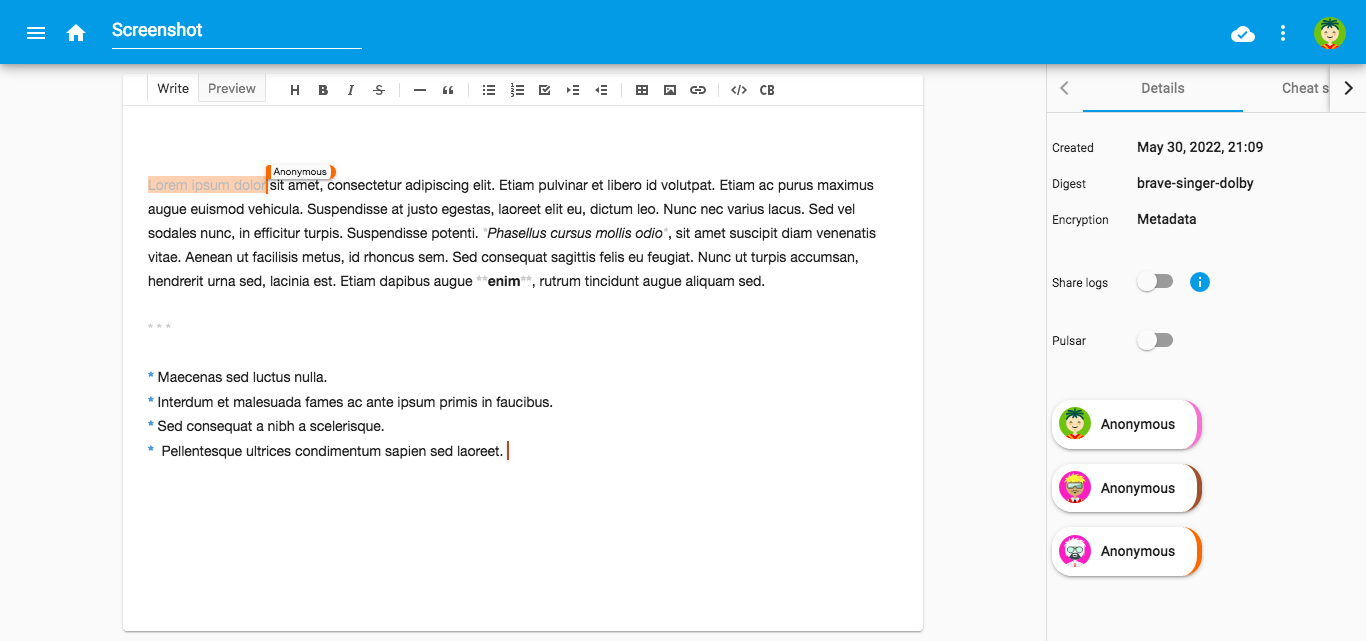
\includegraphics{img/screenshot-mute-editor.png}
        }
    \end{figure}
    \vspace{-0.5cm}
    \begin{itemize}
        \item Application pair-à-pair
        \item Permet de rédiger collaborativement des documents texte
        \item Garantit la confidentialité \& souveraineté des données
    \end{itemize}
\end{frame}

\begin{frame}[fragile]{Réplication dans applications collaboratives pair-à-pair}
    \begin{figure}
        \resizebox{0.7 \textwidth}{!}{
            \begin{tikzpicture}
                \newcommand{\doc}{
                    \tikz{
                        \fill[scale=.15,fill=white,draw=gray,thick,solid] (0,0) -- (7,0) -- (7,8) -- (5,10) -- (0,10) -- cycle;
                    }
                }
                \newcommand{\updsquare}{
                    \tikz{
                        \fill[\colorblockone, scale=.12] (0,0) rectangle (3,3);
                    }
                }
                \newcommand{\updcircle}{
                    \tikz{
                        \fill[\colorblocktwo, scale=.07] (3,3) circle (3);
                    }
                }
                \newcommand{\updtriangle}{
                    \tikz{
                        \fill[\colorblockfive, scale=.07] (0,0) -- (6,0) -- (3,6) -- cycle;
                    }
                }
                \path
                    node[label=90:{A}] (a) {
                        \includegraphics[scale=0.4, page=5, trim=0cm 24cm 32cm 0cm, clip]{img/mute-figures.pdf}
                    }
                    +(-70:3) node[label=-90:{B}] (b) {
                        \includegraphics[scale=0.4, page=5, trim=0cm 24cm 32cm 0cm, clip]{img/mute-figures.pdf}
                    }
                    +(200:4) node[label=-90:{C}] (c) {
                        \includegraphics[scale=0.4, page=5, trim=0cm 24cm 32cm 0cm, clip]{img/mute-figures.pdf}
                    };

                \path
                    (a) node[label={[xshift=2em]0:{\doc}}] {}
                    (b) node[label={[xshift=2em]0:{\doc}}] {}
                    (c) node[label={[xshift=-2em]180:{\doc}}] {};

                \onslide<4->{
                    \path
                        (a) node[label={[xshift=3.8em]90:{\updsquare}}] {}
                        (b) node[label={[xshift=3.7em]0:{\updtriangle}}] {}
                        (c) node[label={[xshift=-4.8em]-90:{\updcircle}}] {};
                }

                \onslide<5->{
                    \draw[dotted] (a) -- (b);
                }

                \only<6>{
                    \path
                        (a) -- node[midway]{
\includegraphics[scale=0.4]{img/sync.pdf}} (b);
                }

                \onslide<7->{
                    \path
                        (a) node[label={[xshift=3.7em]0:{\updtriangle}}] {}
                        (b) node[label={[xshift=3.8em]90:{\updsquare}}] {};
                }

                \onslide<8->{
                    \draw[dotted] (a) -- (c);
                    \draw[dotted] (b) -- (c);
                }

                \only<8> {
                    \path
                        (a) -- node[midway]{
\includegraphics[scale=0.4]{img/sync.pdf}} (c)
                        (b) -- node[midway]{
\includegraphics[scale=0.4]{img/sync.pdf}} (c);
                }

                \onslide<9->{
                    \path
                        (a) node[label={[xshift=3.8em]-90:{\updcircle}}] {}
                        (b) node[label={[xshift=3.8em]-90:{\updcircle}}] {}
                        (c) node[label={[xshift=-4.8em]90:{\updsquare}}] {}
                        (c) node[label={[xshift=-4.8em]0:{\updtriangle}}] {};
                }
            \end{tikzpicture}
        }
    \end{figure}
    \vspace{-1em}
    \begin{columns}
        \hspace{0em}
        \begin{column}{0.6\textwidth}
            \begin{itemize}
                \item<2-> Noeuds peuvent être \alert{déconnectés}
                \item<3-> Doivent pouvoir \alert{travailler sans coordination synchrone} préalable (par ex. consensus)
            \end{itemize}
        \end{column}
        \begin{column}{0.6\textwidth}
            \begin{itemize}
                \item<9-> Doit garantir \alert{cohérence à terme} \cite{10.1145/224057.224070}\dots
                \item<9-> \dots malgré ordres différents d'intégration des modifications
            \end{itemize}
        \end{column}
    \end{columns}
    \onslide<10>{
        \vspace{1em}
        \begin{center}
            \alert{Nécessite des \emph{mécanismes de résolution de conflits}}
        \end{center}
    }
\end{frame}

% \begin{frame}{Évaluation de MUTE}
%     \metroset{block=transparent}
%     \begin{block}{Taille du texte comparée à taille de la séquence répliquée}
%         \begin{columns}
%             \begin{column}{0.6\textwidth}
%                 \begin{figure}
%                     \resizebox{\columnwidth}{!}{
%                         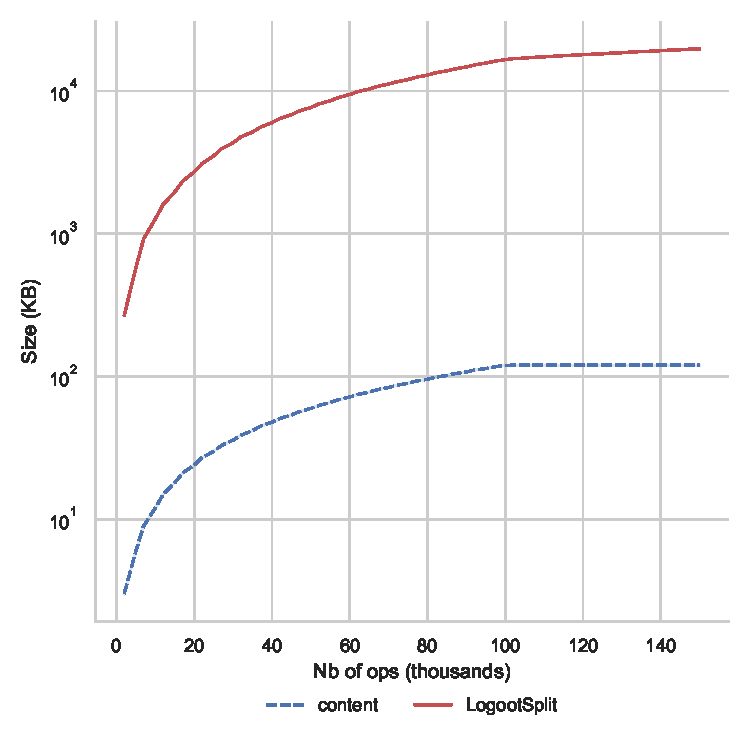
\includegraphics{img/ls-vs-content-snapshot-sizes-7k5.pdf}
%                     }
%                 \end{figure}
%             \end{column}
%             \begin{column}{0.4\textwidth}
%                 \pause
%                 \begin{block}{Constat}
%                     \begin{itemize}
%                         \item 1\% contenu\dots
%                         \item \dots 99\% métadonnées
%                     \end{itemize}
%                 \end{block}
%                 \pause
%                 \begin{center}
%                     \alert{Et ça augmente !}
%                 \end{center}
%                 \pause
%                 \begin{block}{Impact}
%                     \begin{itemize}
%                         \item Surcoût \alert{mémoire}\dots
%                         \item \dots mais aussi surcoût en \alert{calculs} et en \alert{bande-passante}
%                     \end{itemize}
%                 \end{block}
%             \end{column}
%         \end{columns}
%     \end{block}
% \end{frame}

% \begin{frame}[standout]
%     Comment peut-on \alert{réduire le surcoût} des mécanismes de résolution de conflits dans les applications pair-à-pair ?
% \end{frame}

\subsection{Conflict-free Replicated Data Types (CRDTs) pour le type Séquence}

\begin{frame}{Conflict-free Replicated Data Types (CRDTs)  \cite{shapiro_2011_crdt}}
    \begin{itemize}
        \item Nouvelles spécifications des types de données, \eg \emph{Ensemble} ou \emph{Séquence}
        \item Incorpore nativement mécanisme de résolution de conflits
    \end{itemize}
    \pause
    \begin{block}{Propriétés des CRDTs}
        \begin{itemize}
            \item Permettent modifications \alert{sans coordination}
            \item Garantissent la \alert{cohérence forte à terme}
        \end{itemize}
    \end{block}
    \pause
    \begin{block}{Cohérence forte à terme}
        Ensemble des noeuds ayant intégrés le même ensemble de modifications obtient des états équivalents, \alert{sans nécessiter d'actions ou messages supplémentaires}
    \end{block}
\end{frame}

\begin{frame}[fragile]{CRDTs pour le type Séquence}
    \metroset{block=transparent}
    \begin{columns}
        \begin{column}{0.6\textwidth}
            \begin{block}{\quad Type Séquence usuel}
                \begin{figure}[!ht]
                    \centering
                    \resizebox{\columnwidth}{!}{
                        \begin{tikzpicture}
                            \newcommand\initialstate[2]{
                                \path
                                    #1
                                    ++#2
                                    node[letter, label=below:{$0$}] {B}
                                    ++(0:\widthletter) node[letter, label=below:{$1$}] {N}
                                    ++(0:\widthletter) node[letter, label=below:{$2$}] {J}
                                    ++(0:\widthletter) node[letter, label=below:{$3$}] {O};
                            }
                            \newcommand\totoa[2]{
                                \path
                                    #1
                                    ++#2
                                    node[letter, label=below:{$0$}] {}
                                    ++(0:\widthletter) node[letter, label=below:{$1$}] {}
                                    ++(0:\widthletter) node[letter, label=below:{$2$}] {}
                                    ++(0:\widthletter) node[letter, label=below:{$3$}] {}
                                    ++(0:\widthletter) node[letter, label=below:{$4$}] {};
                            }
                            \newcommand\totob[2]{
                                \path
                                    #1
                                    ++#2
                                    node[letter, label=below:{$0$}] {B}
                                    ++(0:\widthletter) node[letter, label=below:{$1$}] {}
                                    ++(0:\widthletter) node[letter, label=below:{$2$}] {N}
                                    ++(0:\widthletter) node[letter, label=below:{$3$}] {J}
                                    ++(0:\widthletter) node[letter, label=below:{$4$}] {O};
                            }
                            \newcommand\totoc[2]{
                                \path
                                    #1
                                    ++#2
                                    node[letter, label=below:{$0$}] {B}
                                    ++(0:\widthletter) node[letter, label=below:{$1$}] {A}
                                    ++(0:\widthletter) node[letter, label=below:{$2$}] {N}
                                    ++(0:\widthletter) node[letter, label=below:{$3$}] {J}
                                    ++(0:\widthletter) node[letter, label=below:{$4$}] {O};
                            }

                            \newcommand\offseta{ (90:1) }

                            \path
                                node {\textbf{A}}
                                ++(0:0.5) node (a) {}
                                +(0:10) node (a-end) {}
                                +(0:1) node[point] (a-initial) {}
                                +(0:6) node (a-ins-a) {}
                                +(0:9) node (a-final) {};

                            \initialstate{(a-initial)}{\offseta};
                            \draw[dotted] (a) -- (a-initial) (a-final) -- (a-end);
                            \only<1>{
                                \draw[->, thick] (a-initial) -- (a-final);
                            }
                            \onslide<2->{
                                \path (a-ins-a) node[point, label=-170:{$\trm{ins}(1, A)$}] {};
                                \draw[->, thick] (a-initial) -- (a-ins-a) -- (a-final);
                            }
                            \only<3>{\totoa{(a-ins-a)}{\offseta}}
                            \only<4>{\totob{(a-ins-a)}{\offseta}}
                            \onslide<5->{\totoc{(a-ins-a)}{\offseta}}
                        \end{tikzpicture}
                    }
                \end{figure}
            \end{block}
        \end{column}
        \begin{column}{0.6\textwidth}
            \onslide<7->{
                \begin{block}{CRDTs pour Séquence}
                    \begin{figure}[!ht]
                        \centering
                        \resizebox{\columnwidth}{!}{
                            \begin{tikzpicture}
                                \newcommand\initialstate[2]{
                                    \path
                                        #1
                                        ++#2
                                        node[letter, label=below:{$\trm{id}_0$}] {B}
                                        ++(0:\widthletter) node[letter, label=below:{$\trm{id}_1$}] {N}
                                        ++(0:\widthletter) node[letter, label=below:{$\trm{id}_2$}] {J}
                                        ++(0:\widthletter) node[letter, label=below:{$\trm{id}_3$}] {O};
                                }
                                \newcommand\totoa[2]{
                                    \path
                                        #1
                                        ++#2
                                        node[letter, label=below:{}] {}
                                        ++(0:\widthletter) node[letter, label=below:{}] {}
                                        ++(0:\widthletter) node[letter, label=below:{}] {}
                                        ++(0:\widthletter) node[letter, label=below:{}] {}
                                        ++(0:\widthletter) node[letter, label=below:{}] {};
                                }
                                \newcommand\totob[2]{
                                    \path
                                        #1
                                        ++#2
                                        node[letter, label=below:{$\trm{id}_0$}] {B}
                                        ++(0:\widthletter) node[letter, label=below:{$?$}] {}
                                        ++(0:\widthletter) node[letter, label=below:{$\trm{id}_1$}] {N}
                                        ++(0:\widthletter) node[letter, label=below:{$\trm{id}_2$}] {J}
                                        ++(0:\widthletter) node[letter, label=below:{$\trm{id}_3$}] {O};
                                }
                                \newcommand\totoc[2]{
                                    \path
                                        #1
                                        ++#2
                                        node[letter, label=below:{$\trm{id}_0$}] {B}
                                        ++(0:\widthletter) node[letter, label=below:{$\trm{id}_{0.5}$}] {A}
                                        ++(0:\widthletter) node[letter, label=below:{$\trm{id}_1$}] {N}
                                        ++(0:\widthletter) node[letter, label=below:{$\trm{id}_2$}] {J}
                                        ++(0:\widthletter) node[letter, label=below:{$\trm{id}_3$}] {O};
                                }

                                \newcommand\offseta{ (90:1) }

                                \path
                                    node {\textbf{A}}
                                    ++(0:0.5) node (a) {}
                                    +(0:10) node (a-end) {}
                                    +(0:1) node[point] (a-initial) {}
                                    +(0:6) node (a-ins-a) {}
                                    +(0:9) node (a-final) {};

                                \initialstate{(a-initial)}{\offseta};
                                \draw[dotted] (a) -- (a-initial) (a-final) -- (a-end);
                                \only<7,8>{
                                    \draw[->, thick] (a-initial) -- (a-final);
                                }
                                \onslide<9->{
                                    \path (a-ins-a) node[point, label=-170:{$\trm{ins}(B \prec A \prec N)$}] {};
                                    \draw[->, thick] (a-initial) -- (a-ins-a) -- (a-final);
                                }
                                \only<9>{\totoa{(a-ins-a)}{\offseta}}
                                \only<10>{\totob{(a-ins-a)}{\offseta}}
                                \onslide<11->{\totoc{(a-ins-a)}{\offseta}}
                            \end{tikzpicture}
                        }
                    \end{figure}
                \end{block}
            }
        \end{column}
    \end{columns}
    \begin{itemize}
        \item<6-> Changements d'indices sont \alert{source de conflits}
        \item<7-> CRDTs assignent des \alert{identifiants de position} \cite{2009-treedoc-preguica} à chaque élément
        \item<7->
            Identifiants permettent d'\alert{ordonner les élements}
            \onslide<8->{
                \begin{equation*}
                    \trm{id}_0 \lid \trm{id}_1 \lid \trm{id}_2 \lid \trm{id}_3
                \end{equation*}
            }
        \vspace{-1.5em}
        \item<10->
            Identifiants appartiennent à un \alert{espace dense}
            \onslide<11->{
                \begin{equation*}
                    \trm{id}_0 \lid \trm{id}_{0.5} \lid \trm{id}_1
                \end{equation*}
            }
    \end{itemize}
    \vspace{-1em}
    \onslide<12->{
        \begin{center}
            \alert{Utilise LogootSplit \cite{2013-logootsplit} comme base}
        \end{center}
    }
\end{frame}

\begin{frame}{Identifiant LogootSplit}
    \metroset{block=transparent}
    \begin{block}{Identifiant}
        \begin{itemize}
            \item Composé d'\alert{un ou plusieurs tuples} de la forme
        \end{itemize}
        \vspace{3em}
        \begin{equation*}
            \tikzmarknode{pos}{pos}^{
                \tikzmarknode{nodeId}{nodeId}~\tikzmarknode{nodeSeq}{nodeSeq}
            }_{\tikzmarknode{offset}{offset}}
        \end{equation*}
        \begin{tikzpicture}[overlay,remember picture,>=stealth,nodes={align=left,inner ysep=1pt},<-]
            % For "pos"
            \path<2-> (pos.north) ++ (0,2em) node[anchor=south east,color=ucl1mdred] (legend-pos){\textbf{position (a-z)}};
            \draw<2-> [color=ucl1mdred](pos.north) |- ([xshift=-0.3ex,color=ucl1mdred] legend-pos.south west);
            % For "nodeId"
            \path<3-> (nodeId.north) ++ (0,2em) node[anchor=south west,color=ucl1mdblue] (legend-nodeid){\textbf{identifiant (A-Z) de l'auteur}};
            \draw<3-> [color=ucl1mdblue](nodeId.north) |- ([xshift=0.3ex,color=ucl1mdblue] legend-nodeid.south east);
            % For "nodeSeq"
            \path<4-> (nodeSeq.south) ++ (0,-2em) node[anchor=north west,color=ucl2dkpurple] (legend-nodeseq){\textbf{numéro de séquence (1-9)}};
            \draw<4-> [color=ucl2dkpurple](nodeSeq.south) |- ([xshift=0.3ex,color=ucl2dkpurple] legend-nodeseq.south east);
        \end{tikzpicture}
    \end{block}
    \onslide<5->{
        \begin{block}{Relation d'ordre $\lid$}
            \begin{itemize}
                \item Se base sur l'\alert{ordre lexicographique sur les éléments des tuples}
            \end{itemize}
        \end{block}
    }
    \onslide<6->{
        \begin{block}{Exemples}
            \begin{equation*}
                \id{
                    \only<8>{\mathbf{d}}
                    \only<6,7,9,10,11,12>{d}
                }{F5}{0}
                \onslide<7->{
                    \lid \id{
                        \only<7,9,10,11,12>{m}
                        \only<8>{\mathbf{m}}
                    }{C1}{
                        \only<7,8,9,11,12>{0}
                        \only<10>{\textbf{0}}
                    }
                }
                \onslide<9->{
                    \lid \id{m}{C1}{
                        \only<9,11,12>{1}
                        \only<10>{\textbf{1}}
                        }
                }
            \end{equation*}
            \onslide<11->{
                \begin{equation*}
                    \id{i}{B1}{0} \lid \only<11>{\quad?\quad} \only<12>{\id{i}{B1}{0}\alert{\id{f}{A1}{0}}} \lid \id{i}{B1}{1}
                \end{equation*}
            }
        \end{block}
    }
\end{frame}

\begin{frame}[fragile]{Bloc LogootSplit}
    \begin{itemize}
        \item Coûteux de stocker les identifiants de chaque élément
    \end{itemize}
    \begin{figure}[!ht]
        \begin{tikzpicture}
            \path
                node[letter, label=below:{$\id{m}{C1}{0}$}] {B}
                ++(0:\widthletter) node[letter, label=below:{$\id{m}{C1}{1}$}] {A}
                ++(0:\widthletter) node[letter, label=below:{$\id{m}{C1}{2}$}] {N}
                ++(0:\widthletter) node[letter, label=below:{$\id{m}{C1}{3}$}] {J}
                ++(0:\widthletter) node[letter, label=below:{$\id{m}{C1}{4}$}] {O};
        \end{tikzpicture}
    \end{figure}
    \pause
    \vspace{-1em}
    \begin{itemize}
        \item Aggrège en un \alert{bloc} les éléments ayant des \alert{identifiants contigus}
    \end{itemize}
    \begin{block}{Identifiants contigus}
        Deux identifiants sont contigus si et seulement si :
        \begin{enumerate}
            \item les deux identifiants sont identiques à l'exception de leur dernier offset
            \item ces deux derniers offsets sont consécutifs
        \end{enumerate}
    \end{block}
    \pause
    \begin{itemize}
        \item Note l'intervalle d'identifiants d'un bloc : $\id{pos}{nodeId~nodeSeq}{begin..end}$
    \end{itemize}
    \begin{figure}[!ht]
        \begin{tikzpicture}
            \path
                node[block, label=below:{$\id{m}{C1}{0..4}$}] {BANJO};
        \end{tikzpicture}
    \end{figure}
\end{frame}

\begin{frame}{Limites de LogootSplit}
    \metroset{block=transparent}
    \begin{block}{Taille du contenu comparée à la taille de la séquence LogootSplit}
        \begin{columns}
            \begin{column}{0.6\textwidth}
                \begin{figure}
                    \resizebox{\columnwidth}{!}{
                        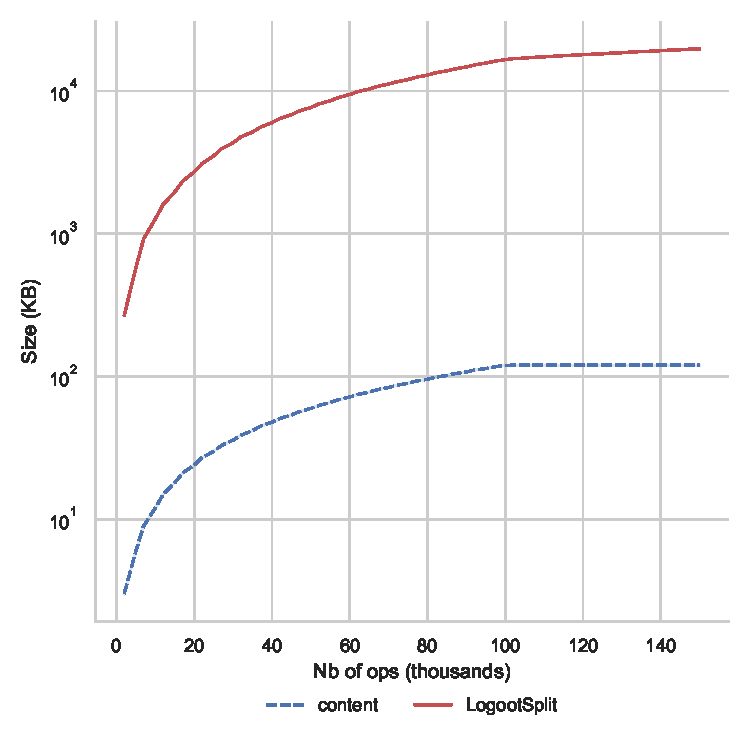
\includegraphics{img/ls-vs-content-snapshot-sizes-7k5.pdf}
                    }
                \end{figure}
            \end{column}
            \begin{column}{0.4\textwidth}
                \pause
                \begin{block}{Constat}
                    \begin{itemize}
                        \item 1\% contenu\dots
                        \item \dots 99\% métadonnées
                    \end{itemize}
                \end{block}
                \pause
                \begin{center}
                    \alert{Et ça augmente !}
                \end{center}
                \pause
                \begin{block}{Impact}
                    \begin{itemize}
                        \item Surcoût \alert{mémoire}\dots
                        \item \dots mais aussi surcoût en \alert{calculs} et en \alert{bande-passante}
                    \end{itemize}
                \end{block}
            \end{column}
        \end{columns}
    \end{block}
\end{frame}

\begin{frame}[standout]
    Comment \alert{réduire le surcoût des CRDTs pour le type Séquence}, dans le cadre de \alert{systèmes pair-à-pair} ?
\end{frame}

% \begin{frame}[fragile]{Proposition}
%     \metroset{block=transparent}
%     \begin{block}{}
%         \begin{figure}
%             \resizebox{\textwidth}{!}{
%               \begin{tikzpicture}
%                 \newcommand\nodeo[1]{
%                     node[letter, label=#1:{$\trm{id}_1$}] {O}
%                 }
%                 \newcommand\noden[1]{
%                     node[letter, label=#1:{$\trm{id}_2$}] {N}
%                 }
%                 \newcommand\nodee[1]{
%                     node[letter, label=#1:{$\trm{id}_3$}] {E}
%                 }
%                 \newcommand\nodeebis[1]{
%                     node[letter, label=#1:{$\trm{id}_{97}$}] {E}
%                 }
%                 \newcommand\nodenbis[1]{
%                     node[letter, label=#1:{$\trm{id}_{98}$}] {N}
%                 }
%                 \newcommand\noded[1]{
%                     node[letter, label=#1:{$\trm{id}_{99}$}] {D}
%                 }


%                 \newcommand\renoneend[1]{
%                     node[block, label=#1:{$\trm{id}'_{begin..end}$}] {ONE$\cdots$END}
%                 }

%                 \newcommand\initialstate[3]{
%                     \path
%                     #1
%                     ++#2
%                     ++(0:0.5)
%                     ++(#3:0.5) \nodeo{-#3}
%                     ++(0:\widthletter) \noden{-#3}
%                     ++(0:\widthletter) \nodee{-#3}
%                     +(0:1.5 * \widthletter) node {$\cdots$}
%                     ++(0:2 * \widthletter) \nodeebis{-#3}
%                     ++(0:\widthletter) \nodenbis{-#3}
%                     ++(0:\widthletter) \noded{-#3};
%                 }

%                 \newcommand\finalstate[3]{
%                   \path
%                   #1
%                   ++#2
%                   ++(0:0.5)
%                   ++(#3:0.5) \renoneend{-#3};
%                 }

%                 \newcommand\offseta{ (90:0.7) }

%                 \path
%                     node {\textbf{A}}
%                     ++(0:0.5) node (a) {}
%                     +(0:11) node (a-end) {}
%                     +(0:1) node[point] (a-initial) {}
%                     +(0:8) node (a-ren) {}
%                     +(0:10) node (a-final) {};

%                 \initialstate{(a-initial)}{\offseta}{90};

%                 \draw[dotted] (a) -- (a-initial) (a-final) -- (a-end);

%                 \only<1,2>{
%                     \draw[->, thick] (a-initial) -- (a-final);
%                 }
%                 \onslide<2->{
%                     \finalstate{(a-ren)}{\offseta}{90};
%                 }
%                 \onslide<3->{
%                     \path (a-ren) node[point, label=-170:{$?$}] {};
%                     \draw[->, thick] (a-initial) --  (a-ren) -- (a-final);
%                 }
%               \end{tikzpicture}
%             }
%           \end{figure}
%           \begin{itemize}
%             \item \alert{Convertir l'état} actuel\dots
%             \item<2-> \dots \alert{en un état optimisé} (identifiants de taille minimale, moins de blocs)\dots
%             \item<3-> \dots à l'aide d'une \alert{nouvelle opération}
%           \end{itemize}
%     \end{block}
% \end{frame}

\subsection{RenamableLogootSplit}

\begin{frame}{Contribution : RenamableLogootSplit}
    \begin{itemize}
        \item CRDT pour le type Séquence qui incorpore un mécanisme de renommage
        \item Réassigne de nouveaux identifiants aux éléments via une nouvelle opération : \ren
    \end{itemize}
    \begin{block}{Propriétés de l'opération \ren}
        \begin{itemize}
            \item Est déterministe
            \item Préserve l'intention des utilisateur-rices
            \item Préserve les propriétés de la séquence, \ie l'unicité et l'ordre de ses identifiants
            \item Est commutative avec les opérations \ins, \rmv mais aussi \ren concurrentes
        \end{itemize}
    \end{block}
\end{frame}

\begin{frame}[fragile]{Opération \ren}
    \begin{figure}
      \resizebox{\textwidth}{!}{
        \begin{tikzpicture}
          \newcommand\nodeh[1]{
              node[letter, label=#1:{$\id{i}{B1}{0}$}] {H}
          }
          \newcommand\nodee[1]{
              node[letter, fill=\colorblockone, label=#1:{$\coloridone\id{i}{B1}{0}\id{f}{A1}{0}$}] {E}
          }
          \newcommand\nodelo[1]{
              node[block, label=#1:{$\id{i}{B1}{1..2}$}] {LO}
          }
          \newcommand\renh[1]{
              node[letter, fill=\colorblocktwo, label=#1:{$\coloridtwo\id{i}{A2}{0}$}] {H}
          }
          \newcommand\rene[1]{
              node[letter, fill=\colorblocktwo, label=#1:{$\coloridtwo\id{i}{A2}{1}$}] {E}
          }
          \newcommand\renl[1]{
              node[letter, fill=\colorblocktwo, label=#1:{$\coloridtwo\id{i}{A2}{2}$}] {L}
          }
          \newcommand\reno[1]{
              node[letter, fill=\colorblocktwo, label=#1:{$\coloridtwo\id{i}{A2}{3}$}] {O}
          }
          \newcommand\renhelo[1]{
              node[block, fill=\colorblocktwo, label=#1:{$\coloridtwo\id{i}{A2}{0..3}$}] {HELO}
          }

          \newcommand\initialstate[3]{
              \path
              #1
              ++#2
              ++(0:0.5)
              ++(#3:0.5) \nodeh{-#3}
              ++(0:\widthletter) \nodee{#3}
              ++(0:\widthletter) \nodelo{-#3};
          }

          \newcommand\stateh[3]{
              \path
              #1
              ++#2
              ++(0:0.5)
              ++(#3:0.5) \renh{-#3};
          }

          \newcommand\statehe[3]{
            \path
            #1
            ++#2
            ++(0:0.5)
            ++(#3:0.5) \renh{-#3}
            ++(0:\widthletter) \rene{-#3};
          }

          \newcommand\statehel[3]{
            \path
            #1
            ++#2
            ++(0:0.5)
            ++(#3:0.5) \renh{-#3}
            ++(0:\widthletter) \rene{-#3}
            ++(0:\widthletter) \renl{-#3};
          }

          \newcommand\statehelo[3]{
            \path
            #1
            ++#2
            ++(0:0.5)
            ++(#3:0.5) \renh{-#3}
            ++(0:\widthletter) \rene{-#3}
            ++(0:\widthletter) \renl{-#3}
            ++(0:\widthletter) \reno{-#3};
          }

          \newcommand\finalstate[3]{
            \path
            #1
            ++#2
            ++(0:0.5)
            ++(#3:0.5) \renhelo{-#3};
          }

          \newcommand\offseta{ (90:0.7) }

          \path
              node {\textbf{A}}
              ++(0:0.5) node (a) {}
              +(0:11) node (a-end) {}
              +(0:1) node[point] (a-initial) {}
              +(0:6) node[point] (a-ren-a1) {}
              +(0:10) node (a-final) {};

          \initialstate{(a-initial)}{\offseta}{90};

          \onslide<1-8>{\path (a-ren-a1) node[label=-170:{$\trm{ren}()$}, label={[xshift=0pt]-10:{$\trm{ren}(A,2)$}}] {};}

          \only<4>{\stateh{(a-ren-a1)}{\offseta}{90}};
          \only<5>{\statehe{(a-ren-a1)}{\offseta}{90};}
          \only<6>{\statehel{(a-ren-a1)}{\offseta}{90};}
          \only<7>{\statehelo{(a-ren-a1)}{\offseta}{90};}
          \onslide<8->{\finalstate{(a-ren-a1)}{\offseta}{90};}

          \draw[dotted] (a) -- (a-initial) (a-final) -- (a-end);
          \draw[->, thick] (a-initial) --  (a-ren-a1) -- (a-final);
        \end{tikzpicture}
      }
    \end{figure}
    \begin{itemize}
      \item<2-> Génère nouvel identifiant pour le 1er élément : \onslide<3->{$\id{i}{B1}{0} \to \id{i}{A2}{0}$}
      \item<4-> Puis génère identifiants contigus pour éléments suivants : \onslide<5->{$\id{i}{A2}{1}$}\onslide<6->{, $\id{i}{A2}{2}$}\onslide<7->{, \dots}
    \end{itemize}

    \onslide<8->{
      \begin{center}
        \alert{Regroupe tous les éléments en 1 unique bloc}
      \end{center}
    }
\end{frame}

\subsection{Intégration des opérations \ins et \rmv concurrentes}

\begin{frame}[fragile]{Interactions avec opérations \ins et \rmv concurrentes}
  \begin{figure}
    \resizebox{\textwidth}{!}{
      \begin{tikzpicture}
        \newcommand\nodeh[1]{
            node[letter, label=#1:{$\id{i}{B1}{0}$}] {H}
        }
        \newcommand\nodee[1]{
            node[letter, fill=\colorblockone, label=#1:{$\coloridone\id{i}{B1}{0}\id{f}{A1}{0}$}] {E}
        }
        \newcommand\nodelo[1]{
            node[block, label=#1:{$\id{i}{B1}{1..2}$}] {LO}
        }
        \newcommand\renhelo[1]{
            node[block, fill=\colorblocktwo, label=#1:{$\coloridtwo\id{i}{A2}{0..3}$}] {HELO}
        }
        \newcommand\nodel[1]{
            node[letter, fill=\colorblockthree, label=#1:{$\coloridthree\id{i}{B1}{0}\id{m}{B2}{0}$}] {L}
        }
        \newcommand\crossl[1]{
            node[letter, cross, fill=\colorblockthree, label=#1:{$\coloridthree\id{i}{B1}{0}\id{m}{B2}{0}$}] {L}
        }

        \newcommand\initialstate[3]{
            \path
                #1
                ++#2
                ++(0:0.5)
                ++(#3:0.5) \nodeh{-#3}
                ++(0:\widthletter) \nodee{#3}
                ++(0:\widthletter) \nodelo{-#3};
        }

        \newcommand\statehelo[3]{
            \path
                #1
                ++#2
                ++(0:0.5)
                ++(#3:0.5) \renhelo{-#3};
        }

        \newcommand\insl[3]{
            \path
            #1
            ++#2
            ++(0:0.5)
            ++(#3:0.5) \nodeh{-#3}
            ++(0:\widthletter) \nodee{#3}
            ++(0:\widthletter) \nodel{-#3}
            ++(0:\widthletter) \nodelo{#3};
        }

        \newcommand\finalstate[3]{
            \path
                #1
                ++#2
                ++(0:0.5)
                ++(#3:0.5) \renhelo{-#3}
                ++(0:\widthblock) \nodel{#3};
        }

        \newcommand\finalstatecrossed[3]{
            \path
                #1
                ++#2
                ++(0:0.5)
                ++(#3:0.5) \renhelo{-#3}
                ++(0:\widthblock) \crossl{#3};
        }

        \newcommand\offseta{ (90:0.7) }
        \newcommand\offsetb{ (-90:0.7) }

        \path
            node {\textbf{A}}
            ++(0:0.5) node (a) {}
            +(0:16) node (a-end) {}
            +(0:1) node[point] (a-initial) {}
            +(0:6) node[point, label=-170:{$\trm{ren}()$}, label={[xshift=0pt]-10:{$\trm{ren}(A,2)$}}] (a-ren-a1) {}
            +(0:12) node (a-recv-ins-l) {}
            +(0:15) node (a-final) {};
        \path<3->
            (a-recv-ins-l) node[point] {};

        \initialstate{(a-initial)}{\offseta}{90};
        \statehelo{(a-ren-a1)}{\offseta}{90};
        \only<4>{\finalstate{(a-recv-ins-l)}{\offseta}{90};}
        \onslide<5->{\finalstatecrossed{(a-recv-ins-l)}{\offseta}{90};}

        \draw[dotted] (a) -- (a-initial) (a-final) -- (a-end);
        \draw<-2>[->, thick] (a-initial) --  (a-ren-a1) -- (a-final);
        \draw<3->[->, thick] (a-initial) --  (a-ren-a1) -- (a-recv-ins-l) -- (a-final);

        \path
            ++(270:2) node {\textbf{B}}
            ++(0:0.5) node (b) {}
            +(0:16) node (b-end) {}
            +(0:1) node[point] (b-initial) {}
            +(0:6) node (b-ins-l) {}
            +(0:15) node (b-final) {};
        \path<2->
            (b-ins-l) node[point, label=170:{$\trm{ins}(E \prec L \prec L)$}] {};
        \path<3->
            (b-ins-l) node[label={[xshift=45pt]10:{$\trm{ins}({\coloridthree\id{i}{B1}{0}\id{m}{B2}{0}},L)$}}] {};

        \initialstate{(b-initial)}{\offsetb}{-90};
        \onslide<2->{\insl{(b-ins-l)}{\offsetb}{-90};}

        \draw[dotted] (b) -- (b-initial) (b-final) -- (b-end);
        \draw<1>[->, thick] (b-initial) -- (b-final);
        \draw<2->[->, thick] (b-initial) --  (b-ins-l) -- (b-final);

        \draw<3->[->, dashed, shorten >= 1] (b-ins-l) -- (a-recv-ins-l);
      \end{tikzpicture}
    }
  \end{figure}
  \begin{itemize}
    \item Noeuds peuvent générer opérations concurrentes aux opérations \ren
    \item<5-> Opérations produisent anomalies si intégrées naïvement
  \end{itemize}
  \onslide<6>{
    \begin{center}
      \alert{Nécessité d'un mécanisme dédié}
    \end{center}
  }
\end{frame}

\begin{frame}{Décomposition de la contribution}
    \begin{block}{Besoins}
        \begin{enumerate}
            \item Détecter les opérations concurrents aux opérations \ren
            \item Prendre en compte les effets des opérations \ren lors de l'intégration des opérations concurrentes
            \pause
            \item Résoudre les conflits provoqués par des opérations \ren concurrentes
            \pause
            \item Supprimer les métadonnées introduites par le mécanisme de renommage lui-même
        \end{enumerate}
    \end{block}
    \pause
    \begin{itemize}
        \item Implémentation disponible à l'adresse suivante : \url{https://github.com/coast-team/mute-structs}
    \end{itemize}
\end{frame}

\subsection{Validation}

\begin{frame}{Objectifs}
  \begin{itemize}
    \item \alert{Montrer que RenamableLogootSplit satisfait la convergence forte}
    \item \alert{Montrer que le mécanisme de renommage améliore les performances} de la séquence répliquée (mémoire, calculs, bande-passante)
  \end{itemize}
  \pause
  \begin{center}
    \alert{Conduite d'une évaluation expérimentale}
  \end{center}
\end{frame}

\begin{frame}[standout]
  \alert{Absence d'un jeu de données de sessions d'édition collaborative}

  \medskip
  \pause
  Mise en place de simulations pour générer un jeu de données
\end{frame}

\begin{frame}{Simulations - Architecture}
  \begin{figure}
    \centering
    \resizebox{0.5 \columnwidth}{!}{
      \begin{tikzpicture}
        \path
          +(90:10) node (a) {\includegraphics[page=5, trim=0cm 24cm 32cm 0cm, clip]{img/mute-figures.pdf}}
          +(-90:10) node (b) {\includegraphics[page=5, trim=0cm 24cm 32cm 0cm, clip]{img/mute-figures.pdf}}
          +(180:5) node (c) {\includegraphics[page=5, trim=0cm 24cm 32cm 0cm, clip]{img/mute-figures.pdf}}
          ++(0:10)
          +(90:10) node (d) {\includegraphics[page=5, trim=0cm 24cm 32cm 0cm, clip]{img/mute-figures.pdf}}
          +(-90:10) node (e) {\includegraphics[page=5, trim=0cm 24cm 32cm 0cm, clip]{img/mute-figures.pdf}}
          +(0:5) node (f) {\includegraphics[page=5, trim=0cm 24cm 32cm 0cm, clip]{img/mute-figures.pdf}};

        \draw[latex-latex, line width=1.5mm]
          (a) edge (b) (a) edge (c) (a) edge (d) (a) edge (e) (a) edge (f)
          (b) edge (c) (b) edge (d) (b) edge (e) (b) edge (f)
          (c) edge (d) (c) edge (e) (c) edge (f)
          (d) edge (e) (d) edge (f)
          (e) edge (f);
      \end{tikzpicture}
    }
  \end{figure}
  \begin{itemize}
    \item \alert{10 noeuds} éditent collaborativement un document
    \item Topologie \alert{réseau entièrement maillée}
    \item Ne considère \alert{pas de pannes ou de pertes de message}
  \end{itemize}
\end{frame}

\begin{frame}{Simulations - Modifications}
  \metroset{block=transparent}
  Noeuds \alert{utilisent LogootSplit} (LS) ou \alert{RenamableLogootSplit} (RLS)
  \pause
  \begin{block}{Se décompose en 2 phases}
    \begin{enumerate}
      \item \alert{Génération du contenu} (80\% d'\ins, 20\% de \rmv)
      \item \alert{Édition} (50/50\%)
    \end{enumerate}
    Noeuds passent à la phase 2 quand leur copie locale atteint une taille donnée (15 pages - 60k caractères)
  \end{block}
  \pause
  \textbf{Nombre d'opérations : } 15k par noeud, 150k au total
\end{frame}

\begin{frame}{Simulations - Mécanisme de renommage}
  \metroset{block=transparent}
  \begin{block}{Noeuds de renommage}
    \begin{itemize}
      \item 1 à 4 noeuds effectuent une \alert{opération \ren toutes les 30k opérations}
      \item Opérations \ren générées à un point donné sont \alert{concurrentes}
    \end{itemize}
  \end{block}
\end{frame}

\begin{frame}{Simulations - Sorties}
  \begin{itemize}
    \item \alert{Instantané de l'état} de chaque noeud à différents points de la simulation (10k opérations et état final)
    \item \alert{Journal des opérations} de chaque noeud
  \end{itemize}
  \pause
  \begin{center}
    \alert{Permet de conduire évaluations sur ces données}\singlefootnote{Code des simulations et benchmarks : \url{https://github.com/coast-team/mute-bot-random}}
  \end{center}
\end{frame}

\begin{frame}{Publications}
    \begin{itemize}
        \item \textbf{Article de position} : \emph{Efficient renaming in CRDTs}, à Middleware 2018 - 19th ACM/IFIP International Middleware Conference (Doctoral Symposium), Dec 2018, Rennes, France.
        \item \textbf{Article d'atelier} : \emph{Efficient renaming in Sequence CRDTs}, avec Gérald Oster et Olivier Perrin à PaPoC 2020 - 7th Workshop on Principles and Practice of Consistency for Distributed Data, Apr 2020, Heraklion / Virtual, Greece.
        \item \textbf{Article de revue} : \emph{Efficient renaming in Sequence CRDTs}, avec Gérald Oster et Olivier Perrin dans IEEE Transactions on Parallel and Distributed Systems, Institute of Electrical and Electronics Engineers, 2022, 33 (12), pp.3870-3885.
    \end{itemize}
\end{frame}

\begin{frame}[allowframebreaks]{Bibliographie}
    \vspace{1em}
    \printbibliography%
\end{frame}

\section{MUTE}

\begin{frame}{Architecture système de MUTE}
    \vspace{-0.5cm}
    \begin{figure}
        \resizebox{\textwidth}{!}{
            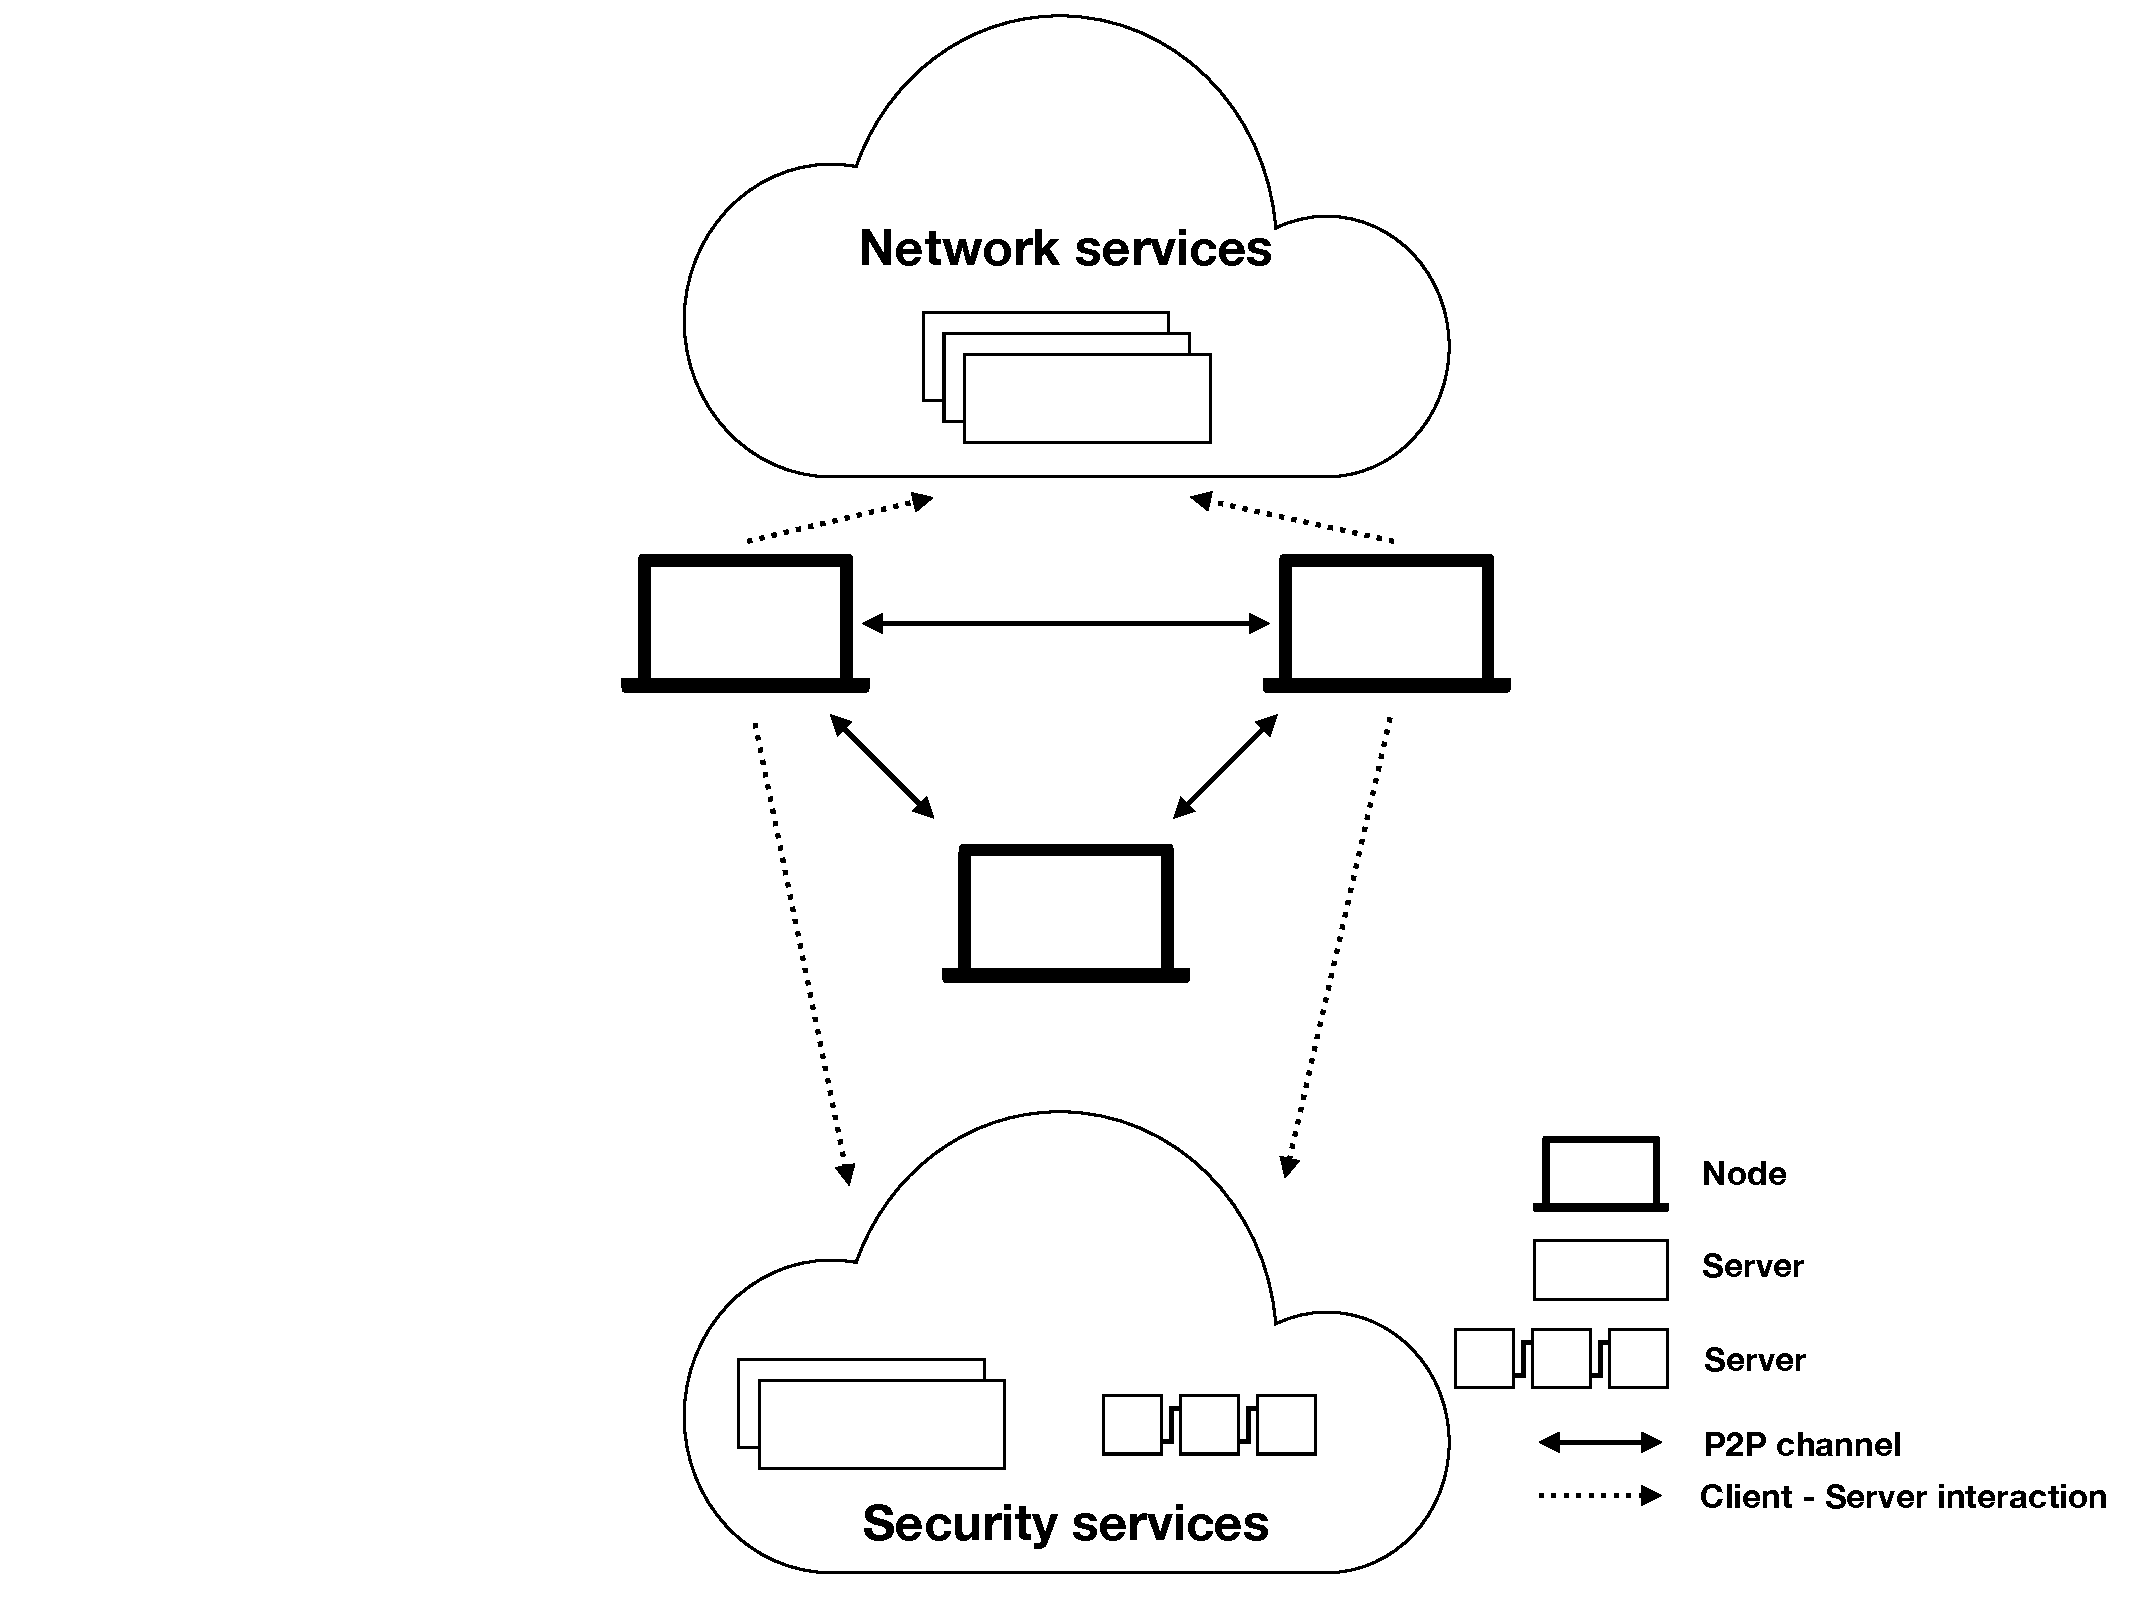
\includegraphics[page=1, trim=0cm 0cm 0cm 0cm, clip, width=.7\linewidth]{img/mute-figures.pdf}
            }
    \end{figure}
\end{frame}


\begin{frame}{Architecture logicielle de MUTE}
    \vspace{-0.5cm}
    \begin{figure}
        \resizebox{\textwidth}{!}{
            \includegraphics[page=2, trim=0cm 0cm 0cm 0cm, clip, width=.7\linewidth]{img/mute-figures.pdf}
        }
    \end{figure}
\end{frame}

\begin{frame}{Contributions}
    \metroset{block=transparent}
    \begin{block}{Document}
        \begin{itemize}
            \item Implémentation des CRDTs LogootSplit et RenamableLogootSplit
        \end{itemize}
    \end{block}

    \begin{block}{Operation Dependancies \& Anti-Entropy}
        \begin{itemize}
            \item Implémentation des modèles de livraison pour LogootSplit et RenamableLogootSplit
            \item Implémentation d'un mécanisme d'anti-entropie (détection et échange des opérations perdues)
        \end{itemize}
    \end{block}

    \begin{block}{Ingénierie logicielle}
        \begin{itemize}
            \item Mise en place des processus d'intégration continue et de livraison continue pour les librairies \texttt{mute-structs}\singlefootnote{\url{https://github.com/coast-team/mute-structs}} et \texttt{mute-core}\singlefootnote{\url{https://github.com/coast-team/mute-core}}
        \end{itemize}
    \end{block}
\end{frame}

\begin{frame}{Contributions - suite}
    \metroset{block=transparent}
    \begin{block}{Network}
        \begin{itemize}
            \item Supervision de la réalisation d'un \emph{Proof of Concept} basé sur l'utilisation d'un \emph{log-based message broker}
        \end{itemize}
    \end{block}

    \begin{block}{Collaborators}
        \begin{itemize}
            \item Supervision de l'adaptation et l'implémentation de SWIM, un protocole d'appartenance au réseau
        \end{itemize}
    \end{block}
\end{frame}


\end{document}
